\chapter{System Design} \label{ch:systemdesign}

\section{System Design} 
% general overview of the system, how every part is integrated, vue app, backend, db, docker etc
In the previous chapter the requirements of the project were illustrated. From these an initial high level overview of the system can be generated as depicted in \autoref{fig:sytemdesign}.

\begin{figure}[H]
    \begin{center}
    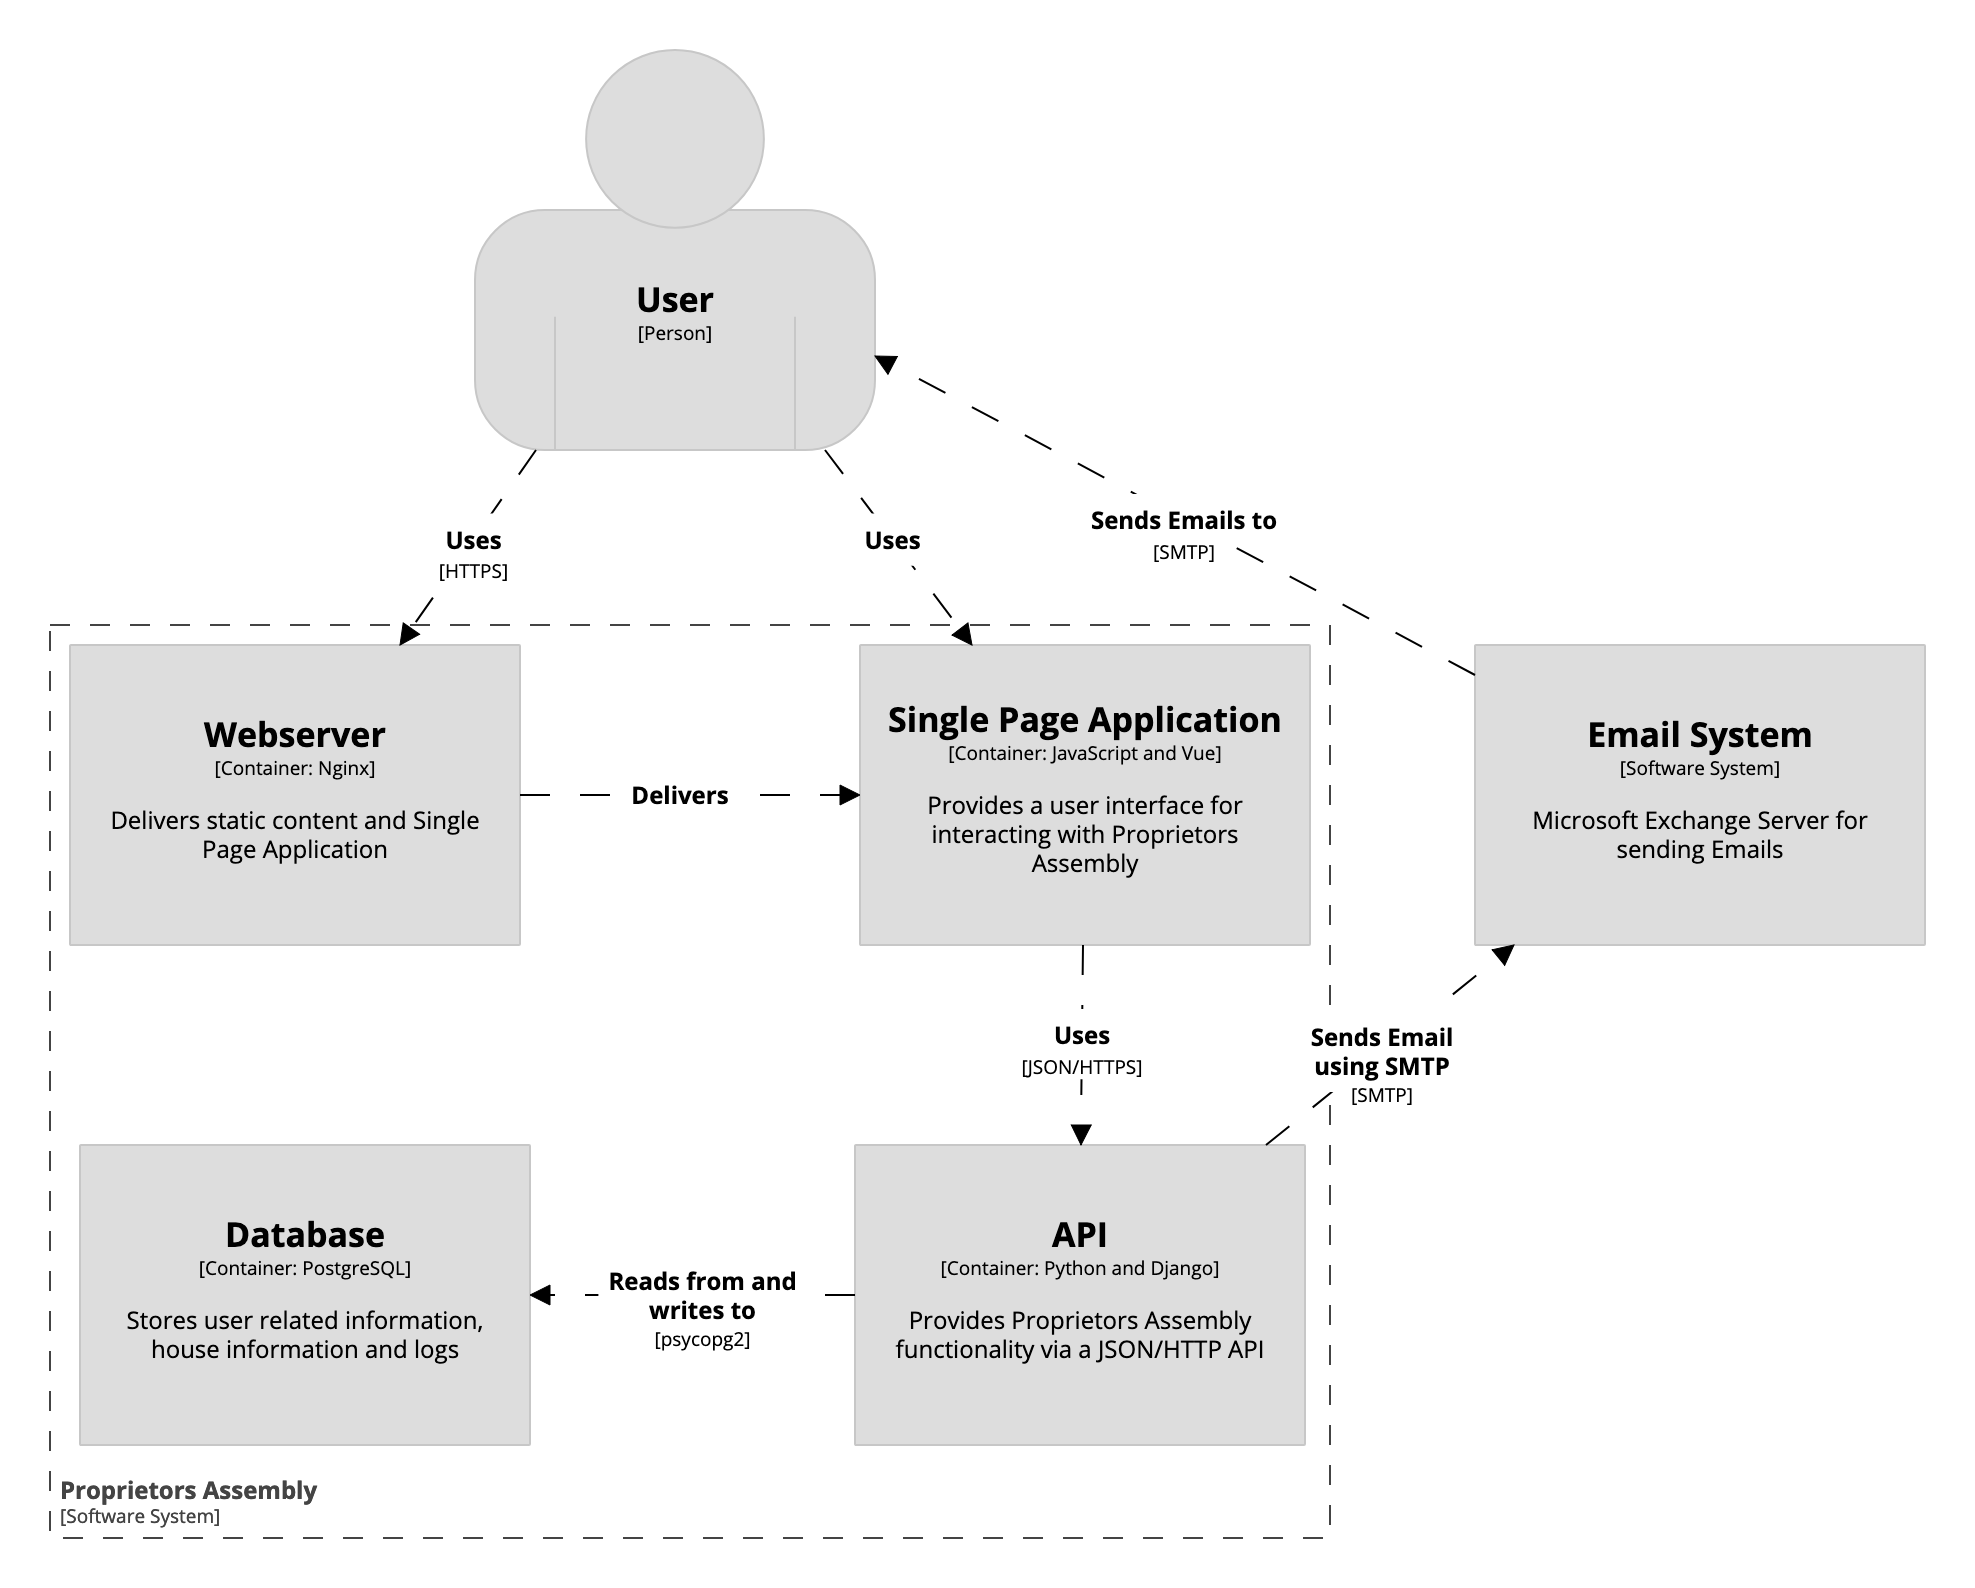
\includegraphics[height=5in]{container_diagram}
    \end{center}
    \caption{System Design}
    \label{fig:sytemdesign}
\end{figure}

In its basic structure, Proprietors Assembly as a software system consists of an NGINX webserver, a Vue \acrlong{spa}, a Django API and a PostgreSQL database. When a user visits the domain \url{https://hausversammlung.at}, the webserver will serve the static frontend which communicates with the API. Depending on the use-case, the API will retrieve data from or add to the Database. An additional third-party Exchange server is used to send emails regarding authentication and house details. The diagram intentionally omitts certain parts of the system for brevity. One of these is a reverse-proxy service which is the first point of contact from a user's viewpoint. A reverse proxy in this case routes between containers which are hosted on the same machine, accessible through unique ports. This topic is discussed in depth in \autoref{ch:deployment}.

\section{Identifying UI Components \& Use Case Flows} \label{sec:uicomponents_flows}
% Defining how to framework should look like, dashboard-like look, what pages have to be created in order to fullfill requirements. Maybe additional wireframes
Interactive components of the frontend are strongly dependant on the required functionality. This section aims to define what is minimally needed on a certain page and to translate functional requirements into identifiable UI elements. This makes it possible to identify elements that are used in multiple places and clearly shows the structure of the frontend. Furthermore, as Vue uses a component-based approach, these elements serve as a tarting point for defining which vue-components are required.

Additionally, as mentioned in \autoref{sec:introplanning} it is the developer's responsibility to derive all use cases and their respective intermediate steps - the use case flow - from the requirements. Since use case flows are very much entangled with how a user interacts with a system and this section is about interactable UI elements, this makes it the most appropriate place to match these. The approach taken is as following: 1) the thought process of what a site should provide is laid out 2) use case flows are derived and UI elements are mapped to a flow 3) all UI elements are noted to analyse which occur multiple times. \textbf{Note:} as too many use case flows would quickly result in a bloated document, only the most important flows per page/category will be shown, additional flows are depicted in \autoref{ch:flows}. 

\subsection{Login Page}
The Login / Register page handles user authentication. A user is required to log into an existing account or create a new one before they can use the system. Traditionally, this is done with a plain HTML-Form. It is sensible to create separate forms for login and register and let the user decide which form to use depending on their needs. Additionally, a forgot-password form should provide a uniform way of requesting a password change. \newline

\begin{table}[H]
  \begin{tabularx}{\linewidth}{|X|}
    \hline
     The user opens the login page or is redirected automatically if not logged in \\
     \hline
     The user provides their email address and password to a form \\
     \hline
     The user clicks "Login" \\
     \hline
     The system checks for appropriate authentication details \\
     \hline
     The user is redirected to the Home page \\
     \hline 
  \end{tabularx}
  \caption{Use Case Flow: Login}
\end{table}

\begin{table}[H]
  \begin{tabularx}{\linewidth}{|X|}
    \hline
     The user opens the login page or is redirected automatically if not logged in \\
     \hline
     The user clicks "Register" \\
     \hline
     The user provides their email address password, firstname and surname to a form \\
     \hline
     The user clicks "Register" \\
     \hline
     The system checks the correctness of the input \\
     \hline
     A new user is added to the system \\
     \hline
     The user is redirected to the Home page \\
     \hline 
  \end{tabularx}
  \caption{Use Case Flow: Register}
\end{table}

Identified Elements: HTML forms for login, register and password-reset

\subsection{Home}
On the home site various data sources should composed into a consolidated view - a dashboard. It shows the most recent forum items, polls and noticeboard entries in addition to the current number of issues, house parties and squaremeters. A user should be able to switch between a list of houses they are associated with. A navigation bar should contain links to all subpages: Home, Noticeboard, Polls, Forum, Issue Management and the Profile. \newline

\begin{table}[H]
  \begin{tabularx}{\linewidth}{|X|}
    \hline
     The user logs in or clicks the Home link in the navigation bar \\
     \hline
     The user is redirected to the Home page \\
     \hline
     The dashboard is shown to the user \\
     \hline
  \end{tabularx}
  \caption{Use Case Flow: View Dashboard}
\end{table}

Identified Elements: Noticeboard Item, Poll Item, Forum Item, House Switcher, Navigation Bar

\subsection{Noticeboard} \label{sub:noticeboardui}
The Noticeboard page contains a list of all noticeboard entries associated with a house. An input field should let the user search for a specific item. A navigation bar as described for the previous page should allow for page changes. Finally, a button that links to a page where noticeboard entries can be created should exist. If the user is the owner of an entry an edit button should be shown. It is sensible to consolidate creating and editing an item on the same site by using a single form which is either initially empty or populated with the existing data should be edited. Creating a noticeboard requires a title and content. \newline

\begin{table}[H]
    \begin{tabularx}{\linewidth}{|X|}
      \hline
       The user opens the noticeboard page by using the navigation bar \\
       \hline
       The user clicks a "create" button \\
       \hline
       The user fills a form with a title and content \\
       \hline
       The system checks for appropriate authorization \\
       \hline
       The system adds a new entry to the database \\
       \hline
       The user is redirected to the main noticeboard page \\
       \hline 
    \end{tabularx}
    \caption{Use Case Flow: Create Noticeboard}
    \label{usecase:createnoticeboard}
  \end{table}
  
Identified Elements: Noticeboard Item List, Noticeboard Item, Search Bar, Navigation Bar, Create Button, Create-Edit Noticeboard Entry Form

\subsection{Polls}
On the Polls page every poll associated with a house is displayed. Users should be provided with a way of searching and filtering these items. A navigation bar should allow for quick page changes. In order to create a poll, users should be shown a button which takes them to a subpage where they can create new polls or edit existing ones. To create a poll, a title and at least two options have to be provided by the user.

\begin{table}[H]
  \begin{tabularx}{\linewidth}{|X|}
    \hline
     The proprietor opens the polls page by using the navigation bar \\
     \hline
     The proprietor clicks a "create" button \\
     \hline
     The proprietor fills a form with a title and poll options \\
     \hline
     The proprietor clicks "Save" \\
     \hline
     The system checks for appropriate authorization \\
     \hline
     The system adds a new entry to the database \\
     \hline
     The proprietor is redirected to the main Polls page \\
     \hline 
  \end{tabularx}
  \caption{Use Case Flow: Create Poll}
\end{table}

Identified Items: Poll Item List, Poll Item, Search Bar, Navigation Bar, Create Button, Create-Edit Poll Form

\subsection{Forum}
The Forum page shows users a list of all thread items of a house which are searchable. A subpage which is accessible by clicking a button should contain a single form for creating and editing items. A thread needs to have a title, category and content. Additionally, a navigation bar links to the other pages.

\begin{table}[H]
  \begin{tabularx}{\linewidth}{|X|}
    \hline
     The user opens the Forum page by using the navigation bar \\
     \hline
     The user clicks a "create" button \\
     \hline
     The user fills a form with a title, question and category \\
     \hline
     The user clicks "Save" \\
     \hline
     The system checks for appropriate authorization \\
     \hline
     The system adds a new entry to the database \\
     \hline
     The user is redirected to the main Forum page \\
     \hline 
  \end{tabularx}
  \caption{Use Case Flow: Create Thread}
\end{table}

Identified Items: Thread Item List, Thread Item, Search Bar, Navigation Bar, Create Button, Create-Edit Thread Form

\subsection{Issue Management}
Similar to the other pages, the issue management page should have a navigation bar, a search bar and a button which links to a subpage where items can be created or edited. Its main purpose is to show a list of all house-related issues. An issue has a reference, date, type, location, title and status.

\begin{table}[H]
  \begin{tabularx}{\linewidth}{|X|}
    \hline
     The user opens the Issues page by using the navigation bar \\
     \hline
     The user clicks a "create" button \\
     \hline
     The user fills a form with a title, category, location and comment \\
     \hline
     The user clicks "Save" \\
     \hline
     The system checks for appropriate authorization \\
     \hline
     The system adds a new entry to the database \\
     \hline
     The user is redirected to the main Issues page \\
     \hline 
  \end{tabularx}
  \caption{Use Case Flow: Log Issue}
\end{table}

Identified Items: Issue Item List, Issue Item, Search Bar, Navigation Bar, Create Button, Create-Edit Issue Form

\subsection{Profile Page}
The profile page provides a way of making changes to a user's account. Initially, they should be able to change their name. Additionally, they should be able to switch languages or house and to invite additional users to their currently active house. \newline

\begin{table}[H]
  \begin{tabularx}{\linewidth}{|X|}
    \hline
     The user opens the Profile page by using the navigation bar \\
     \hline
     The user changes their names \\
     \hline
     The user clicks "Save" \\
     \hline
     The system changes the user's name \\
     \hline 
     The new name is updated throughout the application \\
     \hline 
  \end{tabularx}
  \caption{Use Case Flow: Change Profile Details}
\end{table}


Identified Elements: Language Switcher, Invite Form, House Switcher

\subsection{Add-House Page}
Users need a way of creating a new house or adding an existing house to their account by using an invitation link. To create a new house a form should be provided which takes the address, total squaremeters and role of the user as input variables. An invitation should be accepted by providing an invitation id and the intended role of the user. After creating or accepting an invitation users should be given the possibility to invite additional users to their newly added house. \newline

\begin{table}[H]
\begin{tabularx}{\linewidth}{|X|}
  \hline
   The user clicks "Add House" in the navigation bar \\
   \hline
   The user is redirected to a page where they can add houses \\
   \hline
   The user is presented with two options: Accept Invitation OR Create new House \\
   \hline 
   The user chooses "Accept Invitation" \\
   \hline 
   The user fills a form with invitation id and user role \\
   \hline
   The user clicks "Add" \\
   \hline  
   The system checks if the user is eligible to be added to this house \\
   \hline  
   The user is redirected to a page where they can invite other users to their house \\
   \hline  
\end{tabularx}
\caption{Use Case Flow: Accept Invitation}
\end{table}

Identified Elements: Create House Form, Accept Invite Form, Invite Form

\section{Summary} \label{sec:uisummary}
Some elements are very distinct and are only used once whereas others are used across multiple pages. One element that stands out and is used in almost every single page is the "Navigation Bar". It would be very sensible to not only create a reusable component of this element but to also include it in some kind of base-layout that can be used as a starting point when creating sub-pages. Some other widely used elements are the "Search Bar" and "Create Button". Elements which might not be used very often but reused nevertheless are the "Language Switcher" and "House Switcher". The various forms, lists and items mentioned previously are used only once most of the time and therefore not reused, however, it still makes sense to create reusable Vue components for these to make site composition cleaner and easier.

\section{Site Structure}
Another important aspect of frontend-applications is the question of how the sub-pages are related to one another. This concept can best be described as a sitemap. Well designed sitemaps which are often reflected as links in a navigation bar not only give users a clear understanding of the applications structure but can also be turned into machine-readable files which can be accessed by crawlers. From the previous defined pages it is possible to deduce the complete structure of the frontend-application as depicted in \autoref{fig:sitemap}. \newline
% TODO: Say that create and edit func is on the same site.

\begin{figure}[H]
    \begin{center}
    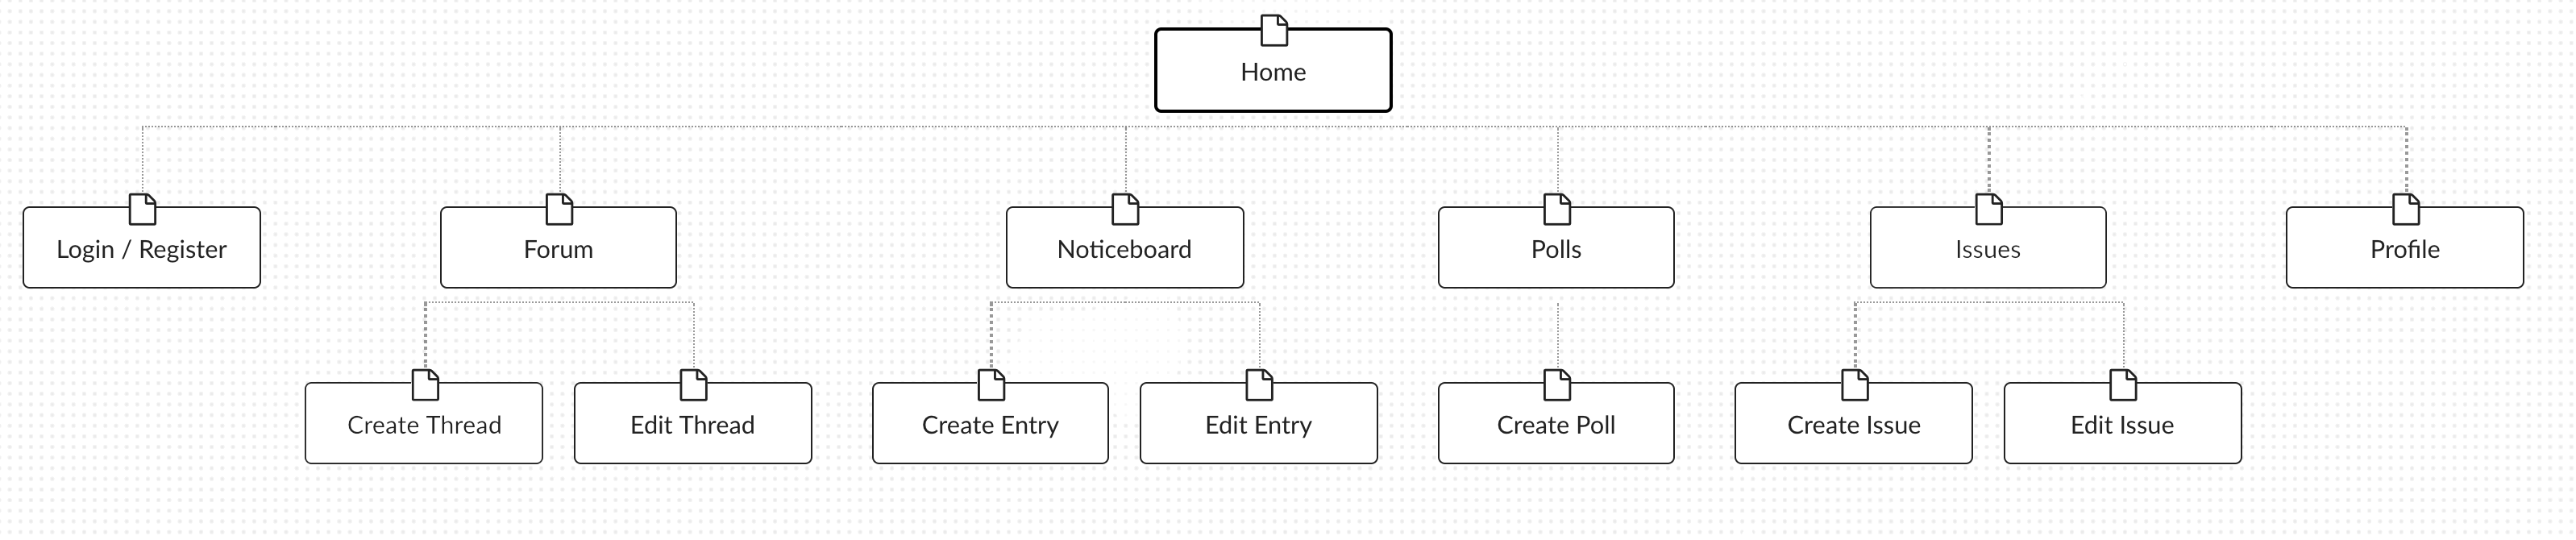
\includegraphics[height=1.8in]{sitemap}
    \end{center}
    \caption{Sitemap}
    \label{fig:sitemap}
\end{figure}